\section{Einleitung}

\subsection{Motivation}

Bei diesem Versuch geht es darum, Methoden der computergesteuerten Datenaufnahme und -verarbeitung kennenzulernen.
Dazu wird die Biegeschwingung eines Metallstäbchens mithilfe elektronischer Verfahren gesteuert und vermessen.
Solche mechanischen Oszillationen werden oft zur Untersuchung der elastischen Eigenschaften von Festkörpern verwendet.
Die näheren physikalischen Eigenschaften und Ergebnisse spielen in diesem Versuch allerdings eine untergeordnete Rolle.
Es handelt sich jedoch um ein gutes Anwendungsbeispiel computergesteuerter Messaufbauten.

Zudem können wir das verwendete Steuerprogramm für die Messinstrumente, LabVIEW, sowie den für die Kommunikation zwischen PC und Geräten zuständigen General Purpose Interface Bus (GPIB) kennenlernen.
Diese Kombination kann durchaus als ein Standard für computergesteuerte Labormessungen verstanden werden und genießt eine entsprechende Bedeutung.

\colorbox{yellow}{TODO Motivation ausführlich genug? Aspekte vergessen?}

\subsection{Physikalische Grundlagen}

\colorbox{yellow}{TODO Was kann man von der Präsentation übernehmen?}

Wobei sich der Amplitudenverlauf $\zeta$ in Abhängigkeit von $\omega$ durch eine Lorentzkurve beschreiben lässt:

\begin{align}
    \label{eq:Lorentzkurve}
    \begin{split}
        \zeta \left( \omega \right) = \frac{f_0}{\sqrt{\left( {\omega_0}^2 - \omega^2 \right)^2 + \gamma^2\omega^2}}
    \end{split}
\end{align}

Ein beispielhafter Verlauf ist in Abbildung \ref{fig:Lorentzkurve} dargestellt.
Das Maximum der Kurve, beschrieben durch Gleichung \ref{eq:Lorentzkurve}, liegt bei der Resonanzfrequenz $\omega = \omega_R := \sqrt{{\omega_0}^2 - \frac{\gamma^2}{2}}$.

\minipage{\linewidth}
    \begin{center}
        \captionsetup{type=figure}
        \begin{adjustbox}{max width=\linewidth, keepaspectratio}
            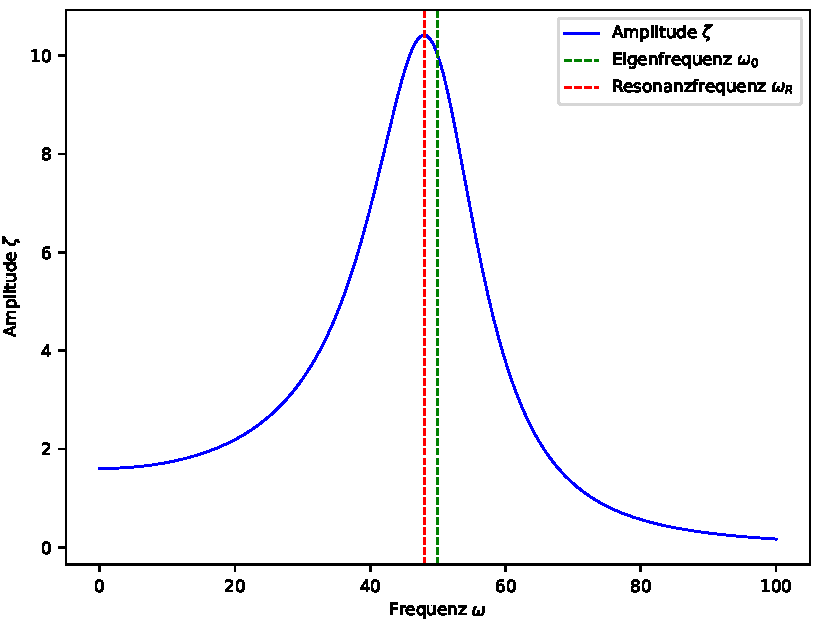
\includegraphics[]{pdf/Lorentzkurve}
        \end{adjustbox}
        \captionof{figure}{Beispielhafter Verlauf einer Lorentzkurve für $f_0 = 10^7$, $\omega_0 = 50$ und $\gamma = 20$ mit eingezeichneten Werten für Eigenfrequenz $\omega_0$ und Resonanzfrequenz $\omega_R$.}
        \label{fig:Lorentzkurve}
    \end{center}
\endminipage

Kraft Kondensatorplatten

\begin{align}
    \label{eq:KraftKondensatorplatten}
    \begin{split}
        F = \frac{C_a U^2}{2 g_a}
    \end{split}
\end{align}

Kapazität Anregungselektrode

\begin{align}
    \label{eq:KapazitaetAnregungselektrode}
    \begin{split}
        C_a = \frac{\varepsilon_0 S}{g_a}
    \end{split}
\end{align}

Periodische Kraft

\begin{align}
    \label{eq:PeriodischeKraft}
    \begin{split}
        F \left( t \right) = \frac{C_a {U_0}^2}{4 g_a} \left( 1 + \cos 2 \omega t \right)
    \end{split}
\end{align}

Kapazität Detektionselektrode

\begin{align}
    \label{eq:KapazitaetDetektionselektrode}
    \begin{split}
        C_d = \frac{\varepsilon_0 S}{g_d}
    \end{split}
\end{align}

Die Spannung der Detektionselektrode lässt sich schreiben als

\begin{align}
    \label{eq:Detektionselektrode}
    \begin{split}
        U_d &= U_B \frac{z}{g_d} \frac{C_d}{C_d + C_L} \frac{\omega R \left( C_d + C_L \right)}{\sqrt{1+\left( \omega R \left( C_d + C_L \right) \right)^2}}
    \end{split}
\end{align}

wobei wir uns zunächst von der Frequenzunabhängigkeit des Übertragungsverhältnisses $\left| \frac{U_d}{z} \right|$ überzeugen sollen.

Dazu kann für den im Experiment verwendeten Frequenzbereich von $\frac{\omega}{2\pi} > \SI{100}{\hertz}$ der letzte Faktor in Gleichung \ref{eq:Detektionselektrode} (entspricht Gleichung 2.6 der Versuchsanleitung \cite{Anleitung}) in guter Näherung durch \SI{1}{} ersetzt werden.
Der Verlauf des Faktors in Abhängigkeit von $\omega$ ist in Abbildung \ref{fig:Faktor} dargestellt.

\minipage{\linewidth}
    \begin{center}
        \captionsetup{type=figure}
        \begin{adjustbox}{max width=\linewidth, keepaspectratio}
            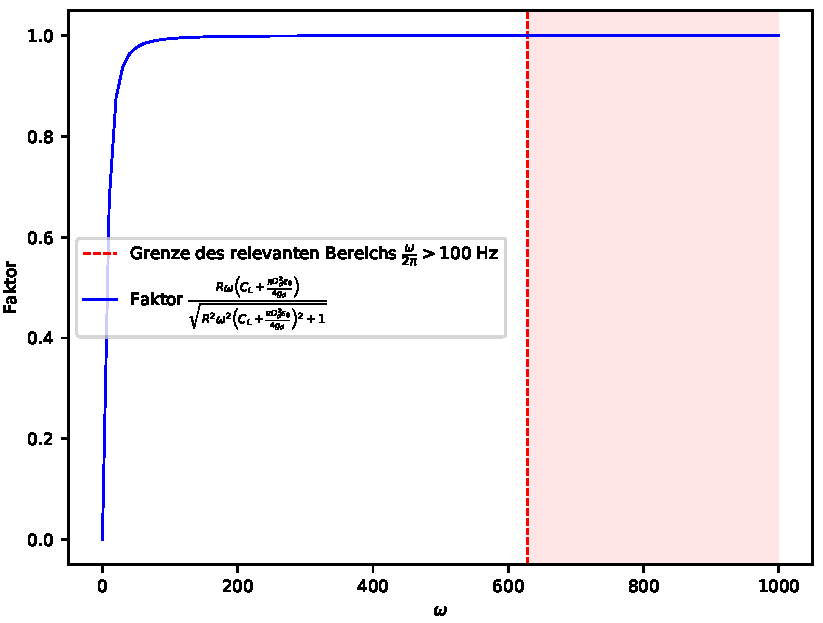
\includegraphics[]{pdf/Faktor}
        \end{adjustbox}
        \captionof{figure}{Letzter Faktor in Gleichung \ref{eq:Detektionselektrode} (entspricht Gleichung 2.6 der Versuchsanleitung \cite{Anleitung}) kann in guter Näherung durch \SI{1}{} ersetzt werden.}
        \label{fig:Faktor}
    \end{center}
\endminipage

Außerdem stellen wir fest, dass $C_d \ll C_L$ und können somit insgesamt schreiben

\begin{align}
    \label{eq:DetektionselektrodeVereinfacht}
    \begin{split}
        \overset{C_d \ll C_L}{\implies} ~~ U_d &\approx U_B \frac{z}{g_d} \frac{C_d}{C_L}
    \end{split}
\end{align}

Diese Beziehung lässt sich also dazu verwenden, zu den im Experiment gemessenen Werten für $U_d$ die entsprechende Auslenkung $z$ der Schwingung zu berechnen.

\subsection{Einige Abschätzungen zur Vorbereitung}

Um uns die Dimensionen des Experiments deutlich zu machen, berechnen wir nun den erwarteten Maximalwert des Amplitudenverlaufs $\zeta$.
Wir nutzen Gleichung 2.8 der Versuchsanleitung

\begin{align}
    \label{eq:MaximaleAmplitude}
    \begin{split}
        \zeta_0 = 4 \frac{l^3}{Ed^3b} F_0
    \end{split}
\end{align}

wobei $F_0$ der Maximalwert der periodischen Anregungskraft nach Gleichung \ref{eq:PeriodischeKraft} ist.

Damit lässt sich nun auch der Maximalwert der Spannung der Detektionselektrode $U_d$ nach Gleichung \ref{eq:DetektionselektrodeVereinfacht} bestimmen.
Wir erhalten für die beiden Werte $\zeta_0 = \SI{2.55}{\nano\meter}$ und $U_{d0} = \SI{5.76}{\micro\volt}$.

Die abgeschätzten Größenordnung unserer Messgrößen bestätigen also die Notwendigkeit des Verstärkers.

\subsection{Theoretische Werte für die erwarteten Eigenfrequenzen}

\colorbox{yellow}{TODO Je nach vorheriger Ausführlichkeit der Einleitung hier noch paar Sätze?}

Mithilfe Gleichung \colorbox{yellow}{TODO} lassen sich die erwarteten Eigenfrequenzen abschätzen.
Das erleichtert uns die spätere Suche nach den tatsächlichen Resonanzkurven während des Experiments.

Wir erhalten $\nu_{0 theo} = \SI{274}{\hertz}$, $\nu_{1 theo} = \SI{1719}{\hertz}$ und $\nu_{2 theo} = \SI{4812}{\hertz}$.

\subsection{Statistische Grundlagen}

\colorbox{yellow}{TODO Grundlagen Fit, chi-squared etc. überhaupt beschreiben oder weglassen?}
